% Generated by ArticleSignalDiagrams. Opaque vector fills only.
\documentclass[10pt,tikz,border=5pt]{standalone}
\usepackage{lmodern}
\usetikzlibrary{fit}
\begin{document}
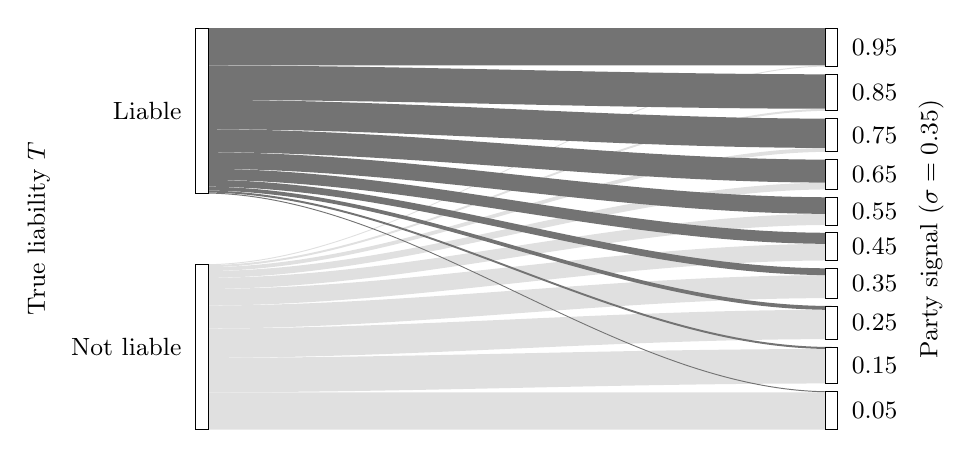
\begin{tikzpicture}[x=1cm,y=1cm,font=\small]\path[fill=black!12,draw=none] (3.3,-5.1) .. controls (6,-5.1) and (8.6,-5.1) .. (11.3,-5.1) -- (11.3,-4.625459) .. controls (8.6,-4.625459) and (6,-4.625459) .. (3.3,-4.625459) -- cycle;
\path[fill=black!12,draw=none] (3.3,-4.625459) .. controls (6,-4.625459) and (8.6,-4.513152) .. (11.3,-4.513152) -- (11.3,-4.075602) .. controls (8.6,-4.075602) and (6,-4.187908) .. (3.3,-4.187908) -- cycle;
\path[fill=black!12,draw=none] (3.3,-4.187908) .. controls (6,-4.187908) and (8.6,-3.950053) .. (11.3,-3.950053) -- (11.3,-3.57806) .. controls (8.6,-3.57806) and (6,-3.815915) .. (3.3,-3.815915) -- cycle;
\path[fill=black!12,draw=none] (3.3,-3.815915) .. controls (6,-3.815915) and (8.6,-3.429156) .. (11.3,-3.429156) -- (11.3,-3.137551) .. controls (8.6,-3.137551) and (6,-3.524311) .. (3.3,-3.524311) -- cycle;
\path[fill=black!12,draw=none] (3.3,-3.524311) .. controls (6,-3.524311) and (8.6,-2.951236) .. (11.3,-2.951236) -- (11.3,-2.740467) .. controls (8.6,-2.740467) and (6,-3.313541) .. (3.3,-3.313541) -- cycle;
\path[fill=black!12,draw=none] (3.3,-3.313541) .. controls (6,-3.313541) and (8.6,-2.5) .. (11.3,-2.5) -- (11.3,-2.359533) .. controls (8.6,-2.359533) and (6,-3.173075) .. (3.3,-3.173075) -- cycle;
\path[fill=black!12,draw=none] (3.3,-3.173075) .. controls (6,-3.173075) and (8.6,-2.048764) .. (11.3,-2.048764) -- (11.3,-1.962449) .. controls (8.6,-1.962449) and (6,-3.08676) .. (3.3,-3.08676) -- cycle;
\path[fill=black!12,draw=none] (3.3,-3.08676) .. controls (6,-3.08676) and (8.6,-1.570844) .. (11.3,-1.570844) -- (11.3,-1.52194) .. controls (8.6,-1.52194) and (6,-3.037855) .. (3.3,-3.037855) -- cycle;
\path[fill=black!12,draw=none] (3.3,-3.037855) .. controls (6,-3.037855) and (8.6,-1.049947) .. (11.3,-1.049947) -- (11.3,-1.024398) .. controls (8.6,-1.024398) and (6,-3.012306) .. (3.3,-3.012306) -- cycle;
\path[fill=black!12,draw=none] (3.3,-3.012306) .. controls (6,-3.012306) and (8.6,-0.486848) .. (11.3,-0.486848) -- (11.3,-0.474541) .. controls (8.6,-0.474541) and (6,-3) .. (3.3,-3) -- cycle;
\path[fill=black!55,draw=none] (3.3,-2.1) .. controls (6,-2.1) and (8.6,-4.625459) .. (11.3,-4.625459) -- (11.3,-4.613152) .. controls (8.6,-4.613152) and (6,-2.087694) .. (3.3,-2.087694) -- cycle;
\path[fill=black!55,draw=none] (3.3,-2.087694) .. controls (6,-2.087694) and (8.6,-4.075602) .. (11.3,-4.075602) -- (11.3,-4.050053) .. controls (8.6,-4.050053) and (6,-2.062145) .. (3.3,-2.062145) -- cycle;
\path[fill=black!55,draw=none] (3.3,-2.062145) .. controls (6,-2.062145) and (8.6,-3.57806) .. (11.3,-3.57806) -- (11.3,-3.529156) .. controls (8.6,-3.529156) and (6,-2.01324) .. (3.3,-2.01324) -- cycle;
\path[fill=black!55,draw=none] (3.3,-2.01324) .. controls (6,-2.01324) and (8.6,-3.137551) .. (11.3,-3.137551) -- (11.3,-3.051236) .. controls (8.6,-3.051236) and (6,-1.926925) .. (3.3,-1.926925) -- cycle;
\path[fill=black!55,draw=none] (3.3,-1.926925) .. controls (6,-1.926925) and (8.6,-2.740467) .. (11.3,-2.740467) -- (11.3,-2.6) .. controls (8.6,-2.6) and (6,-1.786459) .. (3.3,-1.786459) -- cycle;
\path[fill=black!55,draw=none] (3.3,-1.786459) .. controls (6,-1.786459) and (8.6,-2.359533) .. (11.3,-2.359533) -- (11.3,-2.148764) .. controls (8.6,-2.148764) and (6,-1.575689) .. (3.3,-1.575689) -- cycle;
\path[fill=black!55,draw=none] (3.3,-1.575689) .. controls (6,-1.575689) and (8.6,-1.962449) .. (11.3,-1.962449) -- (11.3,-1.670844) .. controls (8.6,-1.670844) and (6,-1.284085) .. (3.3,-1.284085) -- cycle;
\path[fill=black!55,draw=none] (3.3,-1.284085) .. controls (6,-1.284085) and (8.6,-1.52194) .. (11.3,-1.52194) -- (11.3,-1.149947) .. controls (8.6,-1.149947) and (6,-0.912092) .. (3.3,-0.912092) -- cycle;
\path[fill=black!55,draw=none] (3.3,-0.912092) .. controls (6,-0.912092) and (8.6,-1.024398) .. (11.3,-1.024398) -- (11.3,-0.586848) .. controls (8.6,-0.586848) and (6,-0.474541) .. (3.3,-0.474541) -- cycle;
\path[fill=black!55,draw=none] (3.3,-0.474541) .. controls (6,-0.474541) and (8.6,-0.474541) .. (11.3,-0.474541) -- (11.3,-0) .. controls (8.6,-0) and (6,-0) .. (3.3,-0) -- cycle;
\coordinate (axis-midline-0) at (0,-2.55);
\path[fill=white,draw=black,line width=0.3pt] (3.22,-5.1) rectangle (3.38,-3);
\node[anchor=east,fill=white,inner sep=2pt] (bucket-0-0-0) at (3.12,-4.05) {Not liable};
\path[fill=white,draw=black,line width=0.3pt] (3.22,-2.1) rectangle (3.38,-0);
\node[anchor=east,fill=white,inner sep=2pt] (bucket-0-0-1) at (3.12,-1.05) {Liable};
\node[fit=(bucket-0-0-0) (bucket-0-0-1),inner sep=0pt] (source-labels-0) {};
\coordinate (axis-title-0-0) at (source-labels-0.west |- axis-midline-0);
\node[rotate=90,anchor=south,inner sep=0pt] at ([xshift=-0.18cm]axis-title-0-0) {True liability $T$};
\path[fill=white,draw=black,line width=0.3pt] (11.22,-5.1) rectangle (11.38,-4.613152);
\node[anchor=west,fill=white,inner sep=2pt] (bucket-0-1-0) at (11.48,-4.856576) {0.05};
\path[fill=white,draw=black,line width=0.3pt] (11.22,-4.513152) rectangle (11.38,-4.050053);
\node[anchor=west,fill=white,inner sep=2pt] (bucket-0-1-1) at (11.48,-4.281603) {0.15};
\path[fill=white,draw=black,line width=0.3pt] (11.22,-3.950053) rectangle (11.38,-3.529156);
\node[anchor=west,fill=white,inner sep=2pt] (bucket-0-1-2) at (11.48,-3.739605) {0.25};
\path[fill=white,draw=black,line width=0.3pt] (11.22,-3.429156) rectangle (11.38,-3.051236);
\node[anchor=west,fill=white,inner sep=2pt] (bucket-0-1-3) at (11.48,-3.240196) {0.35};
\path[fill=white,draw=black,line width=0.3pt] (11.22,-2.951236) rectangle (11.38,-2.6);
\node[anchor=west,fill=white,inner sep=2pt] (bucket-0-1-4) at (11.48,-2.775618) {0.45};
\path[fill=white,draw=black,line width=0.3pt] (11.22,-2.5) rectangle (11.38,-2.148764);
\node[anchor=west,fill=white,inner sep=2pt] (bucket-0-1-5) at (11.48,-2.324382) {0.55};
\path[fill=white,draw=black,line width=0.3pt] (11.22,-2.048764) rectangle (11.38,-1.670844);
\node[anchor=west,fill=white,inner sep=2pt] (bucket-0-1-6) at (11.48,-1.859804) {0.65};
\path[fill=white,draw=black,line width=0.3pt] (11.22,-1.570844) rectangle (11.38,-1.149947);
\node[anchor=west,fill=white,inner sep=2pt] (bucket-0-1-7) at (11.48,-1.360395) {0.75};
\path[fill=white,draw=black,line width=0.3pt] (11.22,-1.049947) rectangle (11.38,-0.586848);
\node[anchor=west,fill=white,inner sep=2pt] (bucket-0-1-8) at (11.48,-0.818397) {0.85};
\path[fill=white,draw=black,line width=0.3pt] (11.22,-0.486848) rectangle (11.38,-0);
\node[anchor=west,fill=white,inner sep=2pt] (bucket-0-1-9) at (11.48,-0.243424) {0.95};
\node[fit=(bucket-0-1-0) (bucket-0-1-1) (bucket-0-1-2) (bucket-0-1-3) (bucket-0-1-4) (bucket-0-1-5) (bucket-0-1-6) (bucket-0-1-7) (bucket-0-1-8) (bucket-0-1-9),inner sep=0pt] (destination-labels-0) {};
\coordinate (axis-title-0-1) at (destination-labels-0.east |- axis-midline-0);
\node[rotate=90,anchor=north,inner sep=0pt] at ([xshift=0.18cm]axis-title-0-1) {Party signal ($\sigma=0.35$)};
\end{tikzpicture}
\end{document}

